\section{Probabilistic Verification of Network Configuration}\label{sec:NetDice}

\subsection{Introduction}
\begin{table*}
\hbadness 10000
\hfuzz=5pt
  \caption{Properties supported by NetDice}\label{tab:props}
  \begin{center}
    \begin{tabularx}{0.86\textwidth}{c l l}

      & \textbf{Property} & \textbf{Meaning} \\
      \toprule
      \multirow{4}{*}{\rotatebox[origin=c]{90}{Single-Flow}} & $Reach_{u\rightarrow d}$ & Reachability from source $u$ to destination $d$\\ 
      & $Waypoint_{u\rightarrow d}(w)$ & Traffic from $u$ to $d$ traverses $w$ \\
      & $Egress_{u\rightarrow d}(e)$ & Traffic from $u$ to $d$ leaves the network at $e$ \\
      & $PathLength_{u\rightarrow d}(l)$ & Traffic from $u$ to $d$ traverses $l$ links \\

      \hline
      \multirow{3}{*}{\rotatebox[origin=c]{90}{Mutli-Flow}}
      & $Balanced_{F}(\mathcal{L}, \Delta)$ & Under flows $F$ with associated traffic volume, the load
      on the links in $\mathcal{L}$ differs by at most $\Delta$ \\
      & $Isolation_{F}$ & Set of flows in $F$ doesn't share any links \\
      & $Congestion_{F}(l, t)$ & The addition of every traffic from every flow in $F$ do not exceed threshold $t$ for link $l$ \\
	  \bottomrule
    \end{tabularx}
  \end{center}
\end{table*}
% start of the introduction
Ensuring the correctness of network configurations for specific properties (\textit{e.g.}, reachability) in a scalable and precise manner is an important problem interesting ISPs and large companies.
This problem, due to the scale of the deployed networks in such facilities and complex interdependencies between routing protocols, goes beyond the capabilities of current network analysers, as they would have to determine all scenarios for which the property is violated.  
Furthermore, enforcing a property at all times is often not necessary, as the concern is rather on the probability or the fraction of time of that property to holds.
These properties typically emerge from Service Level Agreements (SLAs), defined with respect to a certain metric and holding for a certain fraction of the time.
For example, an ISP could guarantee internet reachability for $99.999\%$ (five 9's) of the time.

To address this problem, we explore the reasoning and the implementation behind NetDice \cite{steffen2020netdice}, a probabilistic verification tool for network configuration. 
It supports modern protocols such as BGP, OSPF and ECMP as well as static routes.
The model of NetDice uses link failures and their probability to compute the probability of a property to hold.  
Such properties typically aim at representing SLAs and can either be expressed with single-flow or multiple-flow considering a flow to be a pair of source and destination IP addresses.
Examples of properties and their meaning are show in Table \ref{tab:props}. 

The key insight of NetDice and the reason for its capacity to handle ISP's network scale is an inference algorithm to efficiently explore link failure scenarios. 
To this end, the concept of cold edges is introduced in Section \ref{sec:HotEdges}.
These edges are used to prune the exploration of failure scenarios as, for a certain configuration, their failures are guaranteed not to change whether a property holds or not.     
The exploration and the corresponding pruning mechanism are explained in Section \ref{sec:explo}. 
To compute the probability of the property to hold, Section \ref{sec:ProbFailMod} details the probability model and the computing method.  
Section \ref{sec:implementation} presents the final implementation. 

Finally, the results of NetDice's usage on synthetic configurations and nation-level ISP are presented (Section \ref{sec:results}).

\subsection{Cold Edges}\label{sec:HotEdges}

This section aims to introduce the concept of cold edges.
Their definition and computation in a local access network (LAN) considering internal static routes and ECMP is initially presented.
Then BGP is incorporated to the model to allow NetDice to reason with external peers.  

As equal-cost multiple path routing (ECMP) is a supported protocol, flows in a network can take multiple paths if they share the same cost.
To represent such behaviour, a forwarding graph, composed of a set of vertices (routers) $V_\textnormal{fwd}$  and a set of directed edges (links) $E_\textnormal{fwd}$, is used.
A forwarding graph can be altered by a link failure representing an unusable link in the configuration, which could be caused by a severed cable or a failing port.  
Multiple link failures form a failure scenario $l$, which is a set containing the unusable links.

\begin{algorithm}[t]
  \floatname{algorithm}{Algorithm}
  \caption{Hot edges for static routes and shortest path}\label{alg:cold}
  \begin{algorithmic}[1]
    \Procedure{HotSpStatic}{u, d, $Static_d$, $E_\textnormal{fwd}$, $l$}
		\State $\mathcal{H} \leftarrow \textnormal{SP}_l(u, d)$ \Comment{initial shortest path}
    \State $\mathcal{S} \leftarrow \{ y ~ | ~ (x, y) \in Static_d ~ \cap ~ E_\textnormal{fwd} \}$ \Comment{end nodes of static route}

		\State $\mathcal{H} \leftarrow \mathcal{H} ~ \cup ~ \textnormal{AllSP}_l(\mathcal{S}, \{d\})$ 
    \State \textbf{return} $\mathcal{H} ~ \cup ~ (Static_d ~ \cap ~ E_\textnormal{fwd})$ 
    \EndProcedure
  \end{algorithmic}
\end{algorithm}

Defining if a property holds in a certain configuration scenario strictly depends on the forwarding graphs, as properties are defined for flows and verified for the internal path used to connect both ends of flows. 
Leveraging the fact that whether a property holds only changes if the forwarding graphs change, NetDice's authors propose the concept of cold and hot edges in Definition \ref{def:cold}.

\begin{definition}\label{def:cold}
  Given a network configuration with a certain failure scenario and a flow $(u, d)$, a subset of edges $\mathcal{C}$ is cold iff any combination of failures in $\mathcal{C}$ is guaranteed not to change the forwarding graph for $(u, d)$. An edge is called cold if it belongs to $\mathcal{C}$ and hot otherwise.
\end{definition}

The separation between cold and hot edges can be used to explore only relevant failure scenarios, as exploring a scenario where the property does not change is redundant.
In practice (Sec. \ref{sec:explo}), hot edges are used to prune the exploration of the possible failure scenarios.
Intuitively, as they impact the forwarding graph, we only explore failure scenarios where hot edges fail to swiftly find scenarios where the property does not hold.
The exploration of cold edges failures is disregarded for a specific scenario, however, it is possible for a cold edge in one scenario to be hot in another (See Fig. \ref{fig:execTree} (D, A) in (16) and (6)).  

{
\hfuzz 30pt
\begin{figure}[t]
	\subfloat{
		\small
		\begin{tabular}[l]{l l}
			\multicolumn{2}{c}{\underline{Application of Alg \ref{alg:cold}}}\\
			2: & $\mathcal{H} = \{(D,E),(E,C)\}$  \\
			3: & $\mathcal{S} = \{B\}$ \\
			4: & $\mathcal{H} = \mathcal{H} \cup \{(B,C)\}$ \\
			5: & $\mathcal{H} = \mathcal{H} \cup \{(E,B)\}$\\
			5: & $\mathcal{H} = \{(D,E),(E,C),(E,B),(B,C)\}$\\
		\end{tabular}
	}
	\subfloat{
		\hspace*{-2cm}
		\vspace*{-2cm}
		
		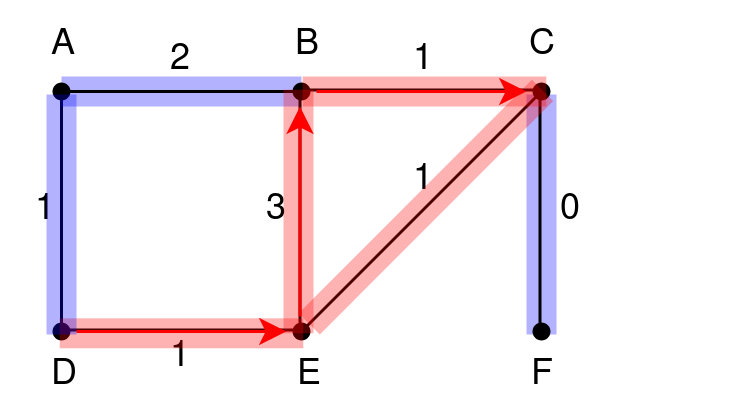
\includegraphics[trim={1cm 1cm 2cm 0.9cm},clip, width=0.45\columnwidth]{figures/ColdStatic.png}
	}
		\caption{This example is from NetDice's article \cite{steffen2020netdice}, it represents cold edges in a network configuration with no failures (i.e. all links up) and a flow (D, C). $(E,B)$ is a static route. Blue and red highlight show cold and hot edges respectively. The forwarding graph is represented by the red arrows.}\label{fig:cold}
\end{figure}
}

\textbf{For a LAN scenario}, an algorithm to compute hot edges considering the shortest paths and  static routes is presented in Alg. \ref{alg:cold}.
It takes a flow $(u,d)$,  the set of static routes $Static_d \subseteq V\times V$ towards a destination $d$, a forwarding graph's edges $E_\textnormal{fwd}$ considering the static routes, and a failure scenario $l$ as parameters. 
The static routes contained in $Static_d = \{(x_i,y_i)\}$ are used by the source $x_i$ to route traffic going towards $d$ to the defined "next-hop" $y_i$.      
This can lead, as discussed below, to the rerouting of the initial shortest path considered by any traversed node, especially the source node of the flow $u$.

Because the property violation depends on forwarding graphs, it is sufficient to consider as hot any edge that may vary the forwarding graph. 
Hence, all edges along the shortest path and the traversed static routes are hot, as a failure in any of them would change whether $\phi$ holds due to unreachability or changes in the forwarding graph. 

To compute the edges along the shortest path we define two algorithms : 
\begin{definition}$\textnormal{SP}_l(s,t)$
	returns the set of all edges along the shortest paths\footnote{Considering ECMP, there might be multiple equal-cost shortest paths} from $s$ to $t$, under link states defined by $l$.
\end{definition}
\begin{definition}$\textnormal{AllSP}_l({\mathcal{S}, \mathcal{T}})$
	returns the union of  $\textnormal{SP}_l(s,t)$ for every source $s \in \mathcal{S}$ to every target $t \in \mathcal{T}$.  
\end{definition} \label{def:allsp}


The algorithm starts by marking as hot every edge along the shortest paths from the source $u$ to the destination $d$ under the failure scenario $l$ (Lin. 2).
This is due to the fact that the shortest path is considered by $u$, so any failure in this shortest path will impact the decision of the source node, hence the resulting forwarding graph.
It holds even if the initially shortest path computed by any source node does not correspond to the final forwarding graph, as static routes can deviate the routing behaviour.
Because any failure along the shortest path, even though it is not used in practice due to the rerouting of the forwarding graph, will change the routing behaviour of the node considering it. 
Finally, every edge on traversed static route is added as hot (Lin.5), as a failure could change the forwarding behaviour.

As an example, Figure \ref{fig:cold} represents the application of Alg \ref{alg:cold} giving the hot and cold edges of a certain network configuration in which : every link is functional, the flow is (D, C), the forwarding edges are $E_\textnormal{fwd} = \{(D,E),(E,B),(B,C)\}$, and the static routes towards are $C$ $Static_C = \{(E,B)\}$.
Note that the $(E,C)$ edge is marked as hot even though it is not in the forwarding graph, because it lies on the shortest path of D.
If it were to fail, the decision of D would be to use $D\rightarrow A\rightarrow B\rightarrow C$ as its shortest path, changing the forwarding graph.  



\begin{table}
	\centering
	\caption{BGP decision process. Announcement are compared in numerical order starting at 1. BGP path attributes are in italic.}\label{tab:bgprocess}
		\begin{tabular}[l]{l l}
			\textbf{Order} & \textbf{Rule}\\
			\hline
			1 & Prefer lowest \textit{local pref} \\
			2 & Prefer Shortest \textit{AS path} \\
			3 & Prefer lowest \textit{origin}  \\
			4 & Prefer lowest \textit{MED} (only compared with same announcer AS) \\
			5 & Prefer external (eBGP) over internal (iBGP) announcements\\
			6 & Prefer lowest IGP cost to BGP "next-hop"\\
			7 & Prefer lowest \textit{BGP peer ID} (tiebreaker) \\
		\end{tabular}
\end{table}

\textbf{Incorporating BGP} is done by considering a flow to be defined by $(u, d)$ with $u$ an internal node and $d$ a BGP destination.
We assume the next-hop for internal routers to be the egress router towards the BGP destination.
NetDice implements a simulation of BGP assuming that all external BGP announcements arrive simultaneously and that the propagation of such announcements is done step-by-step in the network \cite{BGPStepwise}. 
The forwarding graph is computed after the end of the BGP simulation, as the selected next-hop is the next destination of a node towards $d$.

For the simulation, the BGP decision process described in Table \ref{tab:bgprocess} is used.
The implementation of the BGP simulation of NetDice uses route reflectors \cite{rfc4456}.

The definition of cold and hot edges stands when considering BGP.
The key difference BGP makes is the potential change to forwarding graphs occurring if a selected next-hop changes.
There are 3 reasons why a link failure could change the selected next-hop of a node :
\begin{enumerate}
  \item If it causes a disconnection from a BGP peer (which will induce the withdrawal of all routes learned by this peer) 
  \item If the IGP cost towards its current next-hop increases (which could change the decision process of BGP)
  \item The cascading effect of the two above points, as when a node selects another next-hop, it will announce it to its neighbors.
\end{enumerate}

Considering those new possibilities for a forwarding graph to change, the algorithm to compute the hot edges have to assess two properties. (i) keeping the connectivity between BGP peers and (ii) the IGP costs towards a selected next-hop stay unchanged.
So, in addition to the previous requirements, an edge is now hot if its failure would falsify one of these two properties.


The set of network border routers, route reflectors and external BGP nodes are represented respectively by $B_R$, $R_R$ and $E_{xt}$.\\
The algorithm to compute the set of hot edges considering a certain failure scenario $l$, a flow $(u, d)$ and the forwarding graph $E_\textnormal{fwd}$ is presented in	Alg. \ref{alg.hotbgp}.

To reduce computation costs, only the set of nodes $X$ reachable via IGP by $u$ is considered (Lin.2).
The algorithm uses $\textnormal{ALLSP}$ from Definition \ref{def:allsp} and another algorithm defined in Definition \ref{alg:top3}.

\begin{definition}$\textnormal{Top3}(B_R,X)$\label{alg:top3}
	returns, given subset of nodes $X$ and the border routers $B_R$, the subset of border routers $B_{Rl} \subseteq B_R$ announcing the highest preference routes globally.   
\end{definition}

It is used to filter out of the computation the border routers whose announcement will not be selected because the three first rules are global for a fixed BGP destination, or simply because they do not lie in $X$. 
Its effect can be observed in Figure \ref{fig:hotbgp} (i) at the node C : it was filtered out of the considered border routers because its Local Preference (LP) is lower than A and O's announcements.  

The reasoning of Alg. \ref{alg.hotbgp} is similar to Alg. \ref{alg:cold} with the addition of the consideration for the connectivity and unchanged IGP costs properties.
To make sure that all route reflectors receive the announcements of the border routers, the edges along all the shortest paths between every route reflector and border router is marked hot (Lin.3-5).
Similarly to the first algorithm, we need to mark as hot the edges along the shortest paths of $u$ and the end-nodes of traversed static routes towards their selected next-hop (Lin.6-7).
In addition, the forwarding graph $E_\textnormal{fwd}$ can deviate if two successive nodes along it differ in selected next-hop, as the shortest path of the first might not match the shortest path of the second because their selected next-hop may differ.
To take this deviation into account, the edges along the shortest path of the second node towards its selected next-hop are marked as hot.
Note that, contrary to static traversed routes, the edge connecting the two successive nodes with different selected next-hops isn't manually marked hot, as it lies on the shortest path of the first node.
Finally, the edge case where no route reflectors are reachable by $u$ is handled (Lin.12-13). In this case, the connectivity from $u$ towards every border router is required. So every shortest path from $u$ towards them are considered hot.
The first property (i) is ensured by considering the shortest paths. 
The second one is ensured because lines 5 to 10 make sure of the connectivity in the case of at least one route reflector in $X$. Whereas, the lines 11 and 12 take care of the case where no route reflector lies in $X$.

An example of the application of the algorithm can be found in Figure \ref{fig:hotbgp}. The route reflectors are V and W with respectively \{E, D, C, W\} and \{F, B, H, V\} as their clients. The Border routers are E, A and C. There are no static routes and the flow is (B, E).
After the BGP simulation, the forwarding graph is $B \rightarrow C \rightarrow V \rightarrow E$.
Notice that the B packets leave the network at E and not at A which is B's selected next-hop. This is due to B's shortest path to A ($B \rightarrow C \rightarrow F \rightarrow W \rightarrow A$) which traverses C whose next-hop is E, rerouting B's origin forwarding plan to leave the network at E.


Initially, lines 2-5 give $\mathcal{H} = {(E,V), (V,W), (W,A)}$ to ensure the connectivity between the border routers and the route reflectors (represented in  Figure \ref{fig:hotbgp}(iia)).
Then, Figure \ref{fig:hotbgp}(iib) represents the union of the added hot edges from line 6 to 10. It ensures that every edges that could make the IGP cost change is marked as hot.
The shortest path from B towards its selected next-hop is added in line 6 to ensure that IGP costs towards A stay unchanged. This adds ${(B,C), (C,F), (F,W), (W,A)}$ to the set of hot edges.
There is no static route, so the seventh line doesn't change $\mathcal{H}$.
In line 8, we have that C (and E) is added to $D_{\text{NH}}$ as  (B, C) lies on the forwarding graph and both nodes have different next-hop.
Lines 9 to 10 marks hot the edges along the shortest path of C towards E, adding ${(C,V), (V,E)}$ to the set of hot edges.
The final set is the union of the represented sets of Figure \ref{fig:hotbgp}(iib) and (iia) resulting in $\mathcal{H} = {(V,E), (V,W), (W,A), (C,V), (C,F), (B,C), (F,W)}$ represented in Figure \ref{fig:hotbgp} (iii)

\begin{figure*}[t]
	\centering
    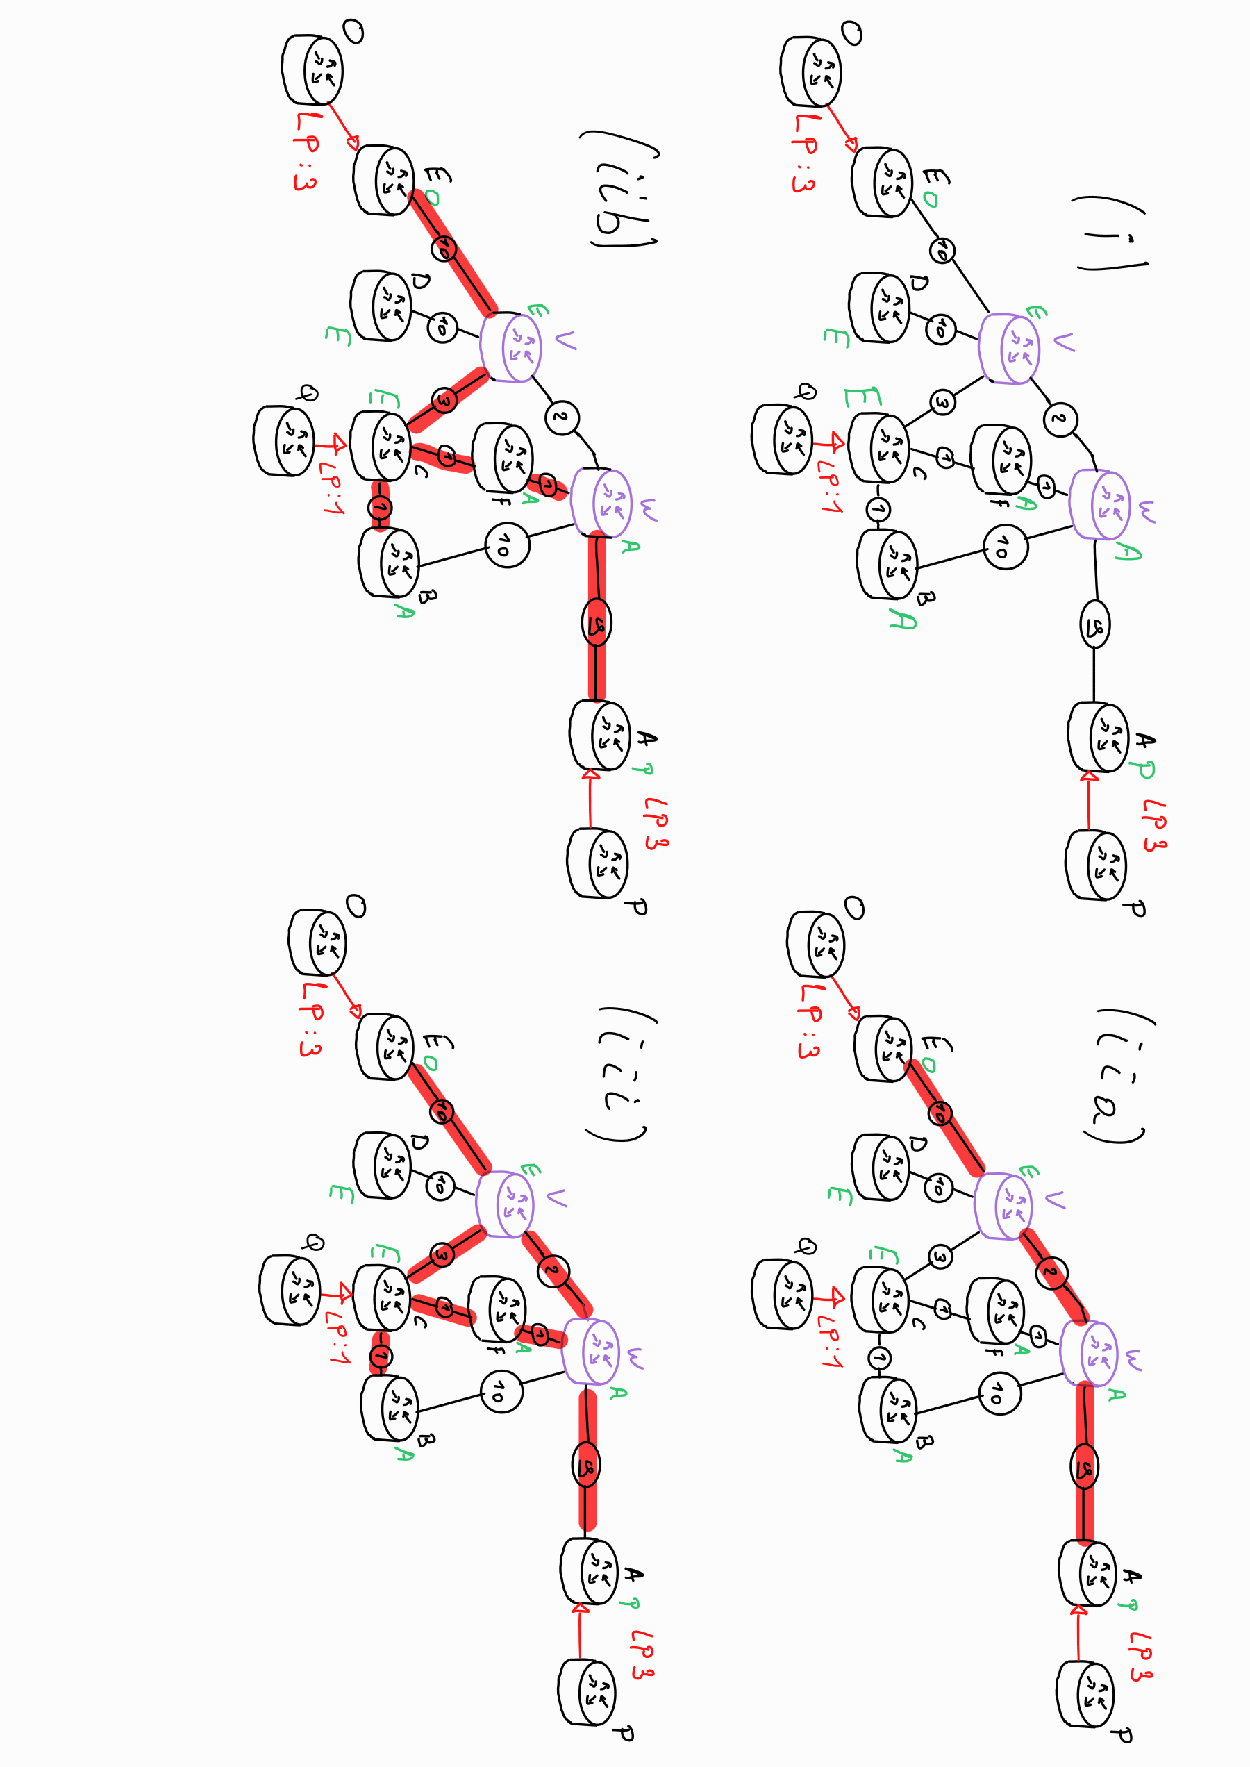
\includegraphics[trim=4cm 0cm 0 0,clip, angle=90,width=0.95\textwidth]{figures/HotBgp.pdf}
	\caption{Computation of hot edges in a BGP capable network configuration.  The flow is $(B,d)$ with d the external BGP destination, LP represents the local preference of the announcements towards d. $B_R = \{E,A,C\}$, $R_R = \{V,W\}$ represented in purple, the selected next-hop is represented in green at each node. Hot edges are highlighted in red.}\label{fig:hotbgp}
\end{figure*}

\begin{algorithm}[t]
  \floatname{algorithm}{Algorithm}
  \caption{Hot edges for BGP}\label{alg.hotbgp}
  \begin{algorithmic}[1]
    \Procedure{HotBGP}{u, d, $E_\textnormal{fwd}$, $l$}

    \State $X \leftarrow$ nodes reachable from $u$ under $l$ 
		\State $B_{Rl} \leftarrow \textnormal{TOP3}(B_R,X)$ \Comment{subset of $B_R$ under consideration of $l$}  
		\State $R_{Rl} \leftarrow R_R \cap X$  \Comment{subset of $R_R$ under consideration of $l$}  
		\State $\mathcal{H} \leftarrow \textnormal{AllSP}_l(R_{Rl}, B_{Rl}, l)$ \Comment{ ensure (i) connectivity}
		\State $\mathcal{H} \leftarrow \mathcal{H} \cup \textnormal{SP}_l(u, \text{NH}_d(u), l)$ \Comment{initial shortest path to next-hop}
    \State $\mathcal{S} \leftarrow \{ y ~ | ~ (x, y) \in Static_d ~ \cap ~ E_\textnormal{fwd} \}$ \Comment{static route}

		\State $\mathcal{D}_{\text{NH}} \leftarrow \{ y ~ | ~ (x, y) \in E_\textnormal{fwd} \wedge \text{NH}_d(x) \neq \text{NH}_d(y) \}$ \Comment{divergent next-hop}

		\For{each $ x \in \mathcal{D}_{\text{NH}} \cup \mathcal{S}$}
		\State $\mathcal{H} \leftarrow \mathcal{H} ~ \cup ~ \textnormal{SP}_l(x, \text{NH}_d(x), l)$ \Comment{ensure (ii) IGP costs unchanged}
    \EndFor


		\If{$R_{Rl} ~ = ~ \emptyset$}
		\State $\mathcal{H} \leftarrow \mathcal{H} \cup \textnormal{AllSP}_l(\{u\}, B_{Rl}, l)$ 
    \EndIf

		\State \textbf{return} $\mathcal{H}$
    \EndProcedure

  \end{algorithmic}
\end{algorithm}


\subsection{Exploration of the failure space}\label{sec:explo}
The exploration of the failure space is achieved by exploring only the possible failures of hot edges. 
To this end, NetDice considers 3 possible states for an edge during the exploration process : 
\begin{itemize}
  \item down : the edge cannot be traversed in current and future scenarios  
  \item up : the edge can be traversed in current and future scenarios  
  \item undefined : the edge is currently traversable but might not be in the future
\end{itemize}

These states are only considered during the exploration process.
In terms of forwarding graph computation, \textit{up} and \textit{undefined} edges are considered traversable whereas \textit{down} edges are not. 
It is assumed that a \textit{check} function returning, given a property and forwarding graphs, whether a property holds in every forwarding graph is implemented for each property.
In practice, it is implemented using variants of DFS depending on the property to check. 
Appendix \ref{app:check} presents an implementation of this \textit{check} function for the waypoint property. 

The exploration procedure can be described as follows : 
\begin{enumerate}
  \item[0)] initially, all edges are undefined (all traversable)
  \item compute the forwarding graphs with respect to the failure scenario
  \item compute the hot edges with the forwarding graphs
  \item let $\mathcal{H}^?$ be the set of undefined hot edges
  \item $\forall h \in \mathcal{H}^?$ make a recursive call (going back to \textit{pt}1) with a failure scenario considering $h$ as down. Once the recursive call is finished (the scenario has been fully explored), set $h$ as up in all future scenarios. 
  % \item return the sum of the recursive calls and the probability of the actual scenario if $\phi$ holds (\textit{check($\phi$)} is true)
\end{enumerate}

Recall that multiple forwarding graphs are possibly computed as equal-cost multi-path is supported.

An example of execution on the network configuration from Figure \ref{fig:cold} with property $\phi =$ "Traffic from D to C traverses E" is shown in Figure \ref{fig:execTree}.

As required, initially all edges are undefined, the hot edges set is computed and recursive calls are made for every hot edge. In the first recursive call (D ${-}\mkern-11mu{/}$ E), we observe that its first recursive call on (A ${-}\mkern-11mu{/}$ D) results in a scenario where C isn't reachable from D. This means that every edge is cold, as any failure would not change the forwarding graph, which is empty.
This leads to a dead end in the exploration, as no more hot edges can be marked as down.
A similar situation happens in the very last recursive call (B ${-}\mkern-11mu{/}$ C), except it's due to a loop in the forwarding graph.
This occurs because E uses its static route and B tries to reach C by E as (B - C) is down.

In the example, only 16 failure scenarios are explored, in contrast to the $2^7 = 128$ scenarios a Brute Force algorithm would have had to explore.


\begin{figure*}[p]
	\centering
	\subfloat{
		\centering
		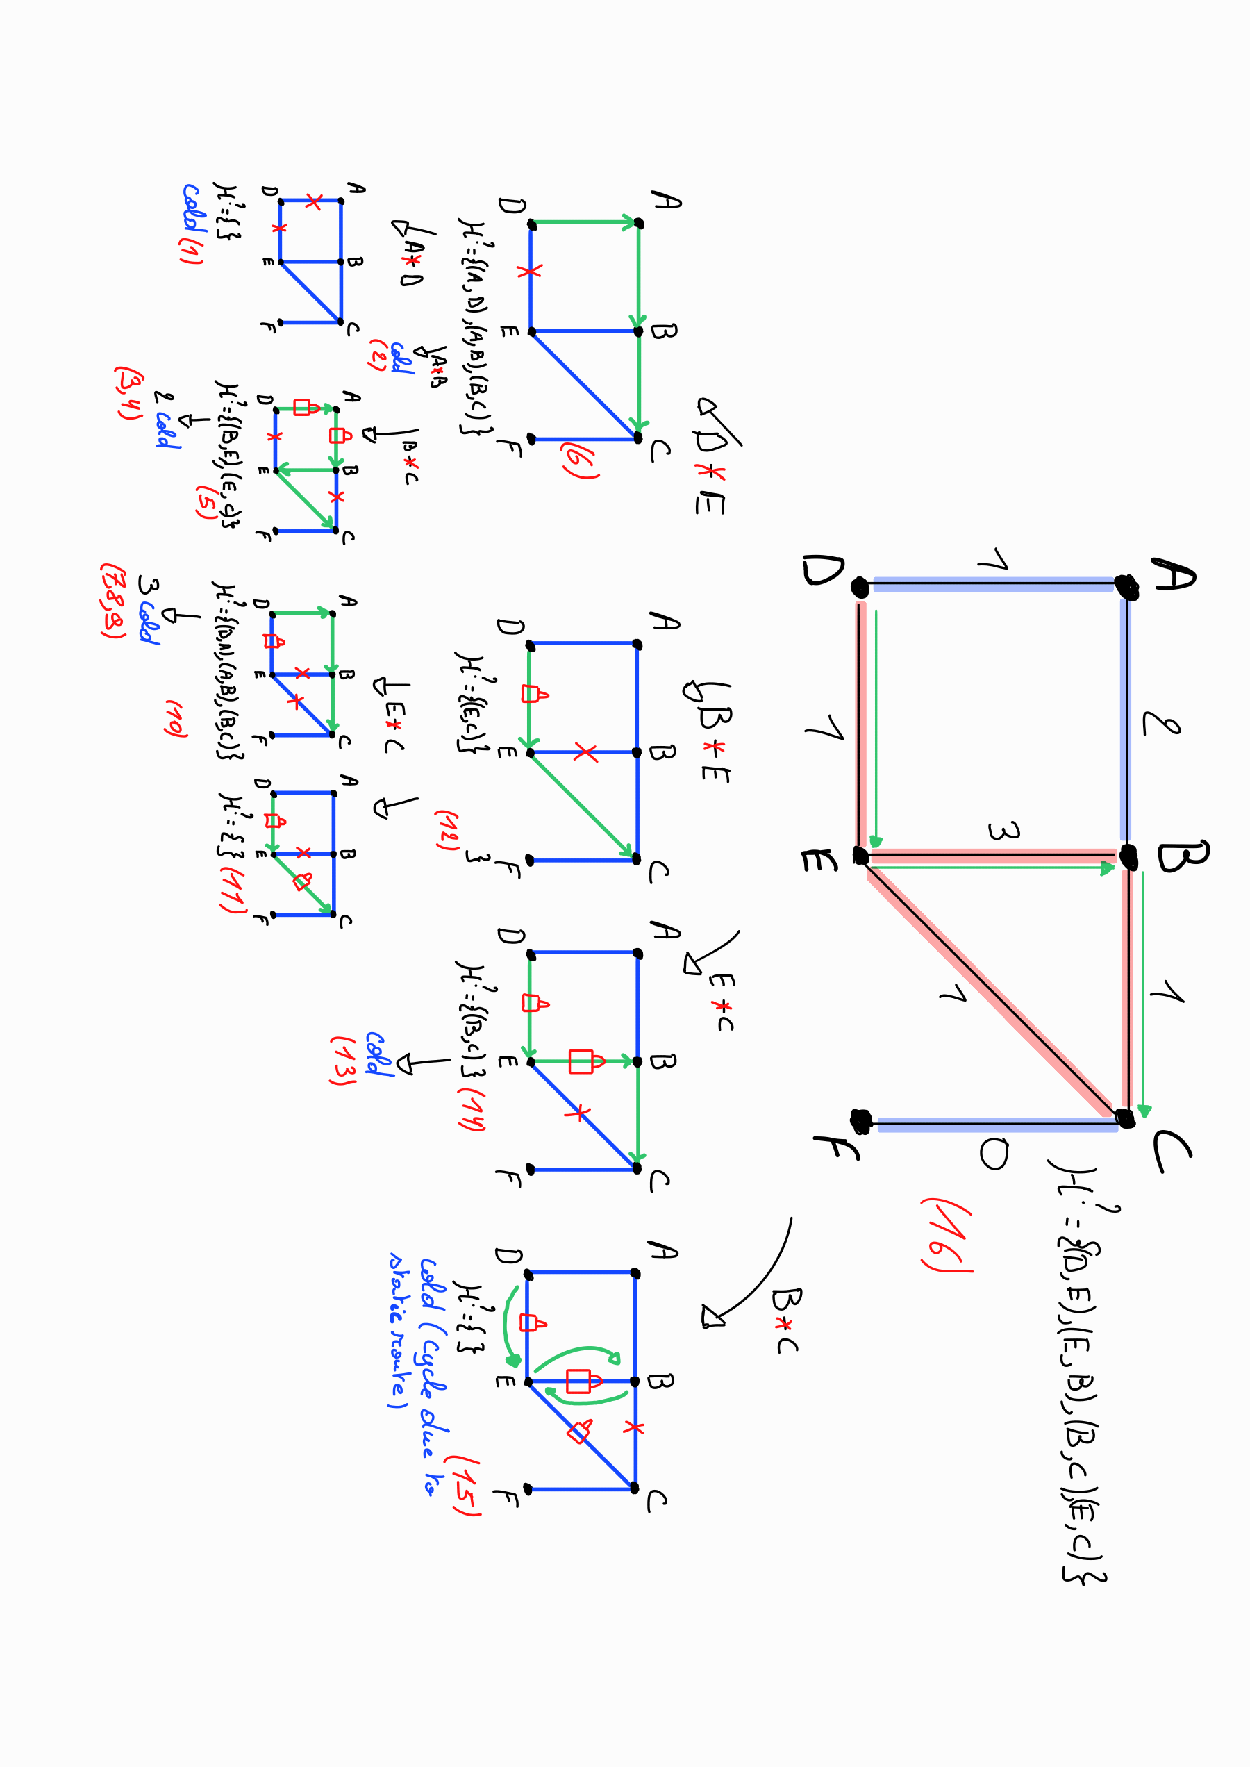
\includegraphics[angle=90,width=0.95\textwidth]{figures/ExplorationWithoutBGP.pdf}
	}
	\hfil
	\subfloat{
		\centering
		\begin{tabular}[l]{l c l}
			\multicolumn{3}{c}{\underline{P($\phi$) with independent probability of link failure p=0.1, $\tilde{p} = 1-p$}}\\
			\textbf{Scenario }&\textbf{Probability returned}&\textbf{Explanation} \\\hline 
			(1,2,3,4):&0 & only cold scenarios\\ 
			(5):&  $\tilde{p}^4*p^2$ & $\phi$ holds with 4 links up and 2 down \\
			(6):&  $\tilde{p}^4*p^2$ & $\phi$ doesn't hold, returns (5)'s result\\
			(7,8,9):&  0 & only cold scenarios\\
			(10):&  0 &  $\phi$ doesn't hold \\
			(11):&  $\tilde{p}^2 * p$ & $\phi$ holds with 2 links up and 1 down \\
			(12):&  $2(\tilde{p}^2 * p)$ & same case as (11) + return of (11) \\
			(13):&  0 &  cold scenario \\
			(14):&  $\tilde{p}^3 * p$ & $\phi$ holds with 3 links up and 1 down \\
			(15):&  0 & cold scenario\\
			(16):&(6)+(12)+(14)+$\tilde{p}^4$& sum of recursive calls, $\phi$ holds \\ 
			\hline
			\multicolumn{3}{l}{\textbf{P($\phi$)} $\approx$ 0.897561}\\
		\end{tabular}
	}
  \caption{On top is the exploration of failure space and on the bottom the computation of the probability with $\phi =$ "Traffic from D to C traverses E". Crosses represent down links, padlocks represent up links and green arrow represent the forwarding graph. Absence of symbol represent undefined links. "Cold" in blue represent scenarios containing only cold edges.}\label{fig:execTree}
\end{figure*}

\subsection{Link Failure Probability model} \label{sec:ProbFailMod}
To compute the probability of a certain failure scenario, two mathematical tools are used :
\begin{enumerate}
  \item A vector $L$ of random variables $s.t.$ $L_e \in \{0,1\}$ for each link $e$ to represent if the link is up ($L_e = 1$) or down ($L_e = 0$) 
  \item A probability mass function of link failure $P(L)$ 
\end{enumerate}
Such that, for a failure scenario represented by a vector $l$ assigning every link to up or down, its probability is defined by $P(L = l)$.

A simple distribution assigning to each link $e \in E$ a probability to fail independently resulting in $P(L = l) = \prod_{e \in E} P(L_e = l_e)$ is considered in Figure \ref{fig:execTree}.
In each failure scenario, if the property holds, its probability is computed by multiplying the probability of defined link states (rather up, down or hot which are considered up).
Then, the returned probability is the sum of the current scenario's probability and the probability of the explored scenario.

\textbf{A more complex probability distribution} $P(L)$, capable of modeling node failures (all incident links) or shared risk link groups (SRLGs), can be represented with  Bayesian Networks.
Because NetDice uses link failure as the baseline for its internal logic, more complex failure models need to be represented by dependencies amongst link failures. For example, a router failure can be modeled by the failure of all its incident links. 
Similarly, the failure of a group of links sharing the same physical resource (shared link risk group or SRLG) is modeled by the failure of the links in the group. 
To model such relations, similarly to other works \cite{BN1,BN2}, NetDice uses Bayesian Networks (BN) to represent the distribution $P(L)$. 

A Bayesian network is a directed acyclic graph whose nodes are random variables and edges represent probabilistic dependencies amongst the variables. Hence, to each node is associated a conditional probability given its parents.    

In the case of NetDice, BN variables are binary variables where the value 0 represents failure and 1 the absence of it. To each link is therefore associated a BN variable to represent its potential state. Other variables can be added to represent node or SRLG failures.  

The motivation for using BN to model the distribution is to have a very general and intuitive model.
It is intuitive by its visual representation in a graph and general because it can represent any discrete probability distribution with arbitrary dependencies. In fact, by the chain rule, any joint discrete probability distribution can be decomposed without loss of generality into a product of conditional distributions that a BN models.


\begin{figure}[t]
	\subfloat{
		\centering
		\begin{tikzpicture}[auto, on grid, thick, state/.style={circle, draw=black, minimum width = 1cm}]
			\matrix [ column sep=0.5cm , row sep=1cm, ampersand replacement=\&] 
			 {
				 \& \node[state](B) {B}; \& \\
				\node[state](A) {A}; \& \& \node[state](C) {C};\\
			 };
			 \path(A) edge node {} (B);
			\path(B) edge node {} (C);
		 \end{tikzpicture}
	 }
	\vfil
	\subfloat{
		\centering
		\begin{tikzpicture}[-latex , auto,  on grid, semithick, state/.style={circle, fill=blue!20, draw=black}]
			\begin{scope}[node distance=2.5cm]
				\node[state, left = of B](A) {A}; \node[state, right = of A](B) {B}; \node[state, right = of B](C) {C}; 
				\node[state, below left = of B](AB) {$A-B$}; 
				\node[state, below right = of B](BC) {$B-C$}; 
			\path(A) edge [bend right=10] node {} (AB);
			\path(B) edge [bend left=10] node {} (BC);
			\path(B) edge [] node {} (AB);
			\path(C) edge [bend left=10] node {} (BC);
			\end{scope}
		 \end{tikzpicture}
	 }
	\caption{On the top is a simple network configuration composed of 3 routers. On the bottom lies the Bayesian network modeling node and link failure for the configuration.}\label{fig:BN}
\end{figure}

Figure \ref{fig:BN} represents a simple network configuration with a BN modeling node failures.
Assuming the probability of a node (resp. link) failure is 0.1 (resp. 0.01), it is possible to compute $P(L = l)$ for a certain failure scenario $l$. 
For example to compute $P(L_{A-B} = 1, L_{B-C} = 0)$ the decomposition is the following.
First, both the A and B  nodes must be 1, otherwise, their shared link would be down. As node failures are independent, we consider :
\[P(A = 1) \times P(B = 1) \times P(L_{A-B} = 1 | A=1,B=1) \] 
\[= 0.9^2 \times 0.99 \]

Then 2 scenarios are possible, either C is up or down.

If C is up :
\[P(L_{B-C}=0~|~B=1,C=1) \times P(C =1) = 0.99 \times 0.9\]  

If C is down : 
\[P(L_{B-C}=0~|~B=1,C=0) \times P(C=0) = 1 \times 0.1\]  

Summing the above scenarios gives $0.109$.

Finally, the final probability is given by : 
\[P(L_{A-B} = 1, L_{A-C} = 0) = 0.109 \times 0.9^2 \times 0.99 = 0.0874071\]

To compute $P(L)$ and its marginals efficiently, NetDice uses the algorithm of variable elimination \cite{VE}.


\subsection{Implementation}\label{sec:implementation}

The following Section presents the NetDice's algorithm to compute the probability of a property given a network configuration and a probability distribution. 
The algorithm, presented in Alg \ref{alg:BGPExplo}, uses the notion of states in which a link can be up (1), down (0) or undefined (?).
As previously stated, only the up and undefined links are considered traversable to check if the property holds. 

Three functions are used by the algorithm.
\begin{definition}{$\textnormal{Scenario}(s, T)$} returns the corresponding failure scenario of the state $s$ by setting every undefined link in the subset $T \subseteq E$ to be up.
\end{definition}

\begin{definition}$\textnormal{Check}(\phi~,~(V^1_{fwd},E^1_{fwd}),\dots,(V^n_{fwd},E^n_{fwd}))$
	returns, given a property and a set of forwarding graphs, if the property holds in every forwarding graph.   
\end{definition}

\begin{definition}$\textnormal{Prob}(s)$
	returns, given a scenario $s$ and a probability distribution $P(L = l)$, the marginal probability over the defined states (either up or down), 
	disregarding the undefined links ($s(e) = ?$).
\begin{flalign}
i.e. && P(\wedge_{e \in E ~ \textnormal{s.t. s(e) $\neq$ ?}} L_e = s(e) )&&\phantom{}
\end{flalign}
\end{definition}


As mutli-flow properties are supported, the check function has to work on a set of forwarding graphs.  

The algorithm initialises by computing a forwarding graph per flow in the property and computing its hot edges set (Lin. 3-5).
Then the undefined hot edges, are retrieved (Lin. 6) for the exploration process. 
If the property is satisfied in every forwarding graph, the probability of the actual scenario is computed.
To do so, the probability of the scenario with the undefined hot edges set to 1 is computed (Lin. 7-8).
This is done to consider hot edges as up and disregard the undefined cold links, as regardless of their state, they do not have impact on rather $\phi$ holds or not.
The exploration of the undefined hot edges is done in Lines 10 to 13 and the algorithm returns the sum of the marginal probabilities of explored states where $\phi$ holds. 

\begin{algorithm}[t]
  \floatname{algorithm}{Algorithm}
  \caption{Computing $P(\phi)$}\label{alg:BGPExplo}
  \begin{algorithmic}[1]
    \Procedure{Explore}{s}
		\State $l \leftarrow \textnormal{Scenario}(s, E)$, $\mathcal{H} \leftarrow \emptyset $, $\rho \leftarrow 0$

    \For{each flow $(u_i, d_i) \in flows(\phi)$}  
	\State compute ($V^i_{fwd}$, $E^i_{fwd}$) for $(u_i, d_i)$ under $l$ 

	\State $\mathcal{H} \leftarrow \mathcal{H} ~ \cup ~ \textnormal{HotBGP}(u_i,d_i, E^i_{fwd}, l)$ \Comment{Alg \ref{alg.hotbgp}}
    \EndFor
		\State $\mathcal{H}^? \leftarrow \mathcal{H} ~ \cap ~ \{ e  \in E ~ | e \text{ is undefined in } s\}$


    \If{Check($\phi$, $(V^1_{fwd},E^1_{fwd}), \dots ,(V^n_{fwd},E^n_{fwd})$)}
	\State $\rho \leftarrow  \textnormal{Prob}(\textnormal{Scenario}(s, \mathcal{H}^?))$ 
    \EndIf
    \State $s' \leftarrow s$ 


    \For{$e^? \in \mathcal{H}^?$}  
		\State $\text{set } e^? \text{ as down in } s'$ 

		\State $\rho \leftarrow \rho + \textnormal{Explore}(s')$ 
		\State $\text{set } e^? \text{ as up in } s'$ 
    \EndFor

    \State \textbf{return} $\rho$

  \EndProcedure
  \end{algorithmic}

  \label{alg:finalImpl}
\end{algorithm}

\subsection{Results} \label{sec:results}



\textbf{Synthetic tests} of NetDice's implementation are done on 90 topologies containing between 19 (resp. 50) and 754 (resp. 2 320) nodes (resp. links). 
The weight of every link is set to 1.
The probability of node (resp. link) failure used is 0.0001 (resp. 0.001).
Regarding BGP configurations, as they are not present in the original topologies, synthetic BGP setups with 2 route reflectors and 10 border routers with 2 external peers each is created by selecting random routers to issue these roles. 
External BGP announcements are created to represent the worst case scenario, where the Top3 algorithm does not prune any announcement.
It implies that the number of border routers considered $B_{Rl}$ is maximal, resulting in a large hot set in Lin. 5 of Alg \ref{alg.hotbgp}. 

The runtime measurements by verifying a random waypoint property with a single random flow considering a target imprecision of $10^{-4}$ (representing four 9's).  
NetDice is run 10 times on each topology with new random choices each time to obtain a more diverse sample size.

Figure \ref{fig:netdiceTests} left represents the maximum and median of the 10 runs for each topology.
Although the runtime of larger networks is clearly higher than smaller networks, most of them can be verified within 1h.
Only 18, out of the 90, topologies require at least 1h to be verified. 

A key insight on the runtime is that it is dominated by the Variable Elimination (VE) (Lin. 8 of Alg. \ref{alg:finalImpl}), as removing node failures yields a 5 to 10 factor improvement. 
While this comes at a cost for the expressiveness of the model, the performance could be improved by using more advanced or specialised algorithms.

\textbf{A real world configuration test} is conducted on an undisclosed nation-level ISP configuration comprising around 100 nodes and 180 links.
The test is conducted by verifying a random single-flow waypoint property on 10 runs, with a target imprecision of $10^{-4}$ and the worst-case BGP announcements.  
Figure \ref{fig:netdiceTests} right represents the summary of the test.
Note that the median time of execution is under two minutes, although more experiments should be conducted to ensure the observed efficiency, it is a promising result. 


\begin{figure}[t]
	\subfloat{
	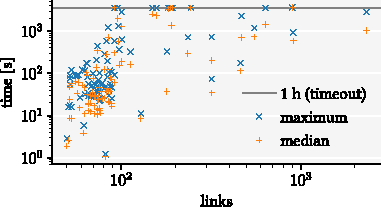
\includegraphics[width=0.70\columnwidth]{figures/netdiceSynth.pdf}
	}
	\subfloat{
	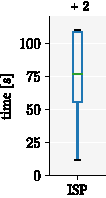
\includegraphics[width=0.24\columnwidth]{figures/netdiceReal.pdf}
	}

	\caption{Runtime for verifying a single-flow waypoint property on synthetic topologies (left) and real ISP configuration (right)}\label{fig:netdiceTests}
\end{figure}


\subsection{Conclusion}
The implementation of NetDice, a scalable probabilistic network configuration verification tool, is presented.

The key insight of the implementation is the introduction of the concept of cold edge.
The manner to retrieve such cold edges are presented considering IGP and BGP protocols.   
This permits the tools to prune the exploration of failure scenarios efficiently.
Moreover, it leverages the modular implementation of Bayesian Networks inference named Variable Elimination (VE) to possibly represent complex failure models.

All the above, although with some inefficiency due to the VE algorithm, enable NetDice to verify properties for small imprecision in a reasonable time as tested on synthetic and real ISP network configurations. 
